
\section{Data and Monte Carlo Simulation}
\subsection{Data Samples}
Brief overview of Full Run 2 and where the data comes from and what time period.\\\\
Luminosity of full run 2. 

\subsection{Monte Carlo Samples}
Signal and Background samples. Choice of cuts at ntuple level. Specifically why each background is chosen (and why others excluded) $\rightarrow$ e.g. talk about branching fractions, cross sections, topology. How are these backgrounds passing our event selection (e.g. ttz $\rightarrow$ b can be lost/untagged/mis-id'ed) $\rightarrow$ provide an explanation for each background.\\\\
Details of each sample (event generator, parton shower).


The following background processes are considered:
\begin{itemize}
	\item $\mathbf{t \bar{t} Z}$: $t \bar{t} $  with an associated $Z$-boson, in the tetralepton final state. Therefore, both top-quarks decay leptonically (e.g. $t \rightarrow W^+ b \rightarrow \ell^+ \nu b$) and of these top-quarks emits a $Z$-boson which decays leptonically ($Z \rightarrow \ell^\pm \ell^\mp$ (OSSF lepton pair) ). This results in a final state with 4 leptons and 2 b-quarks.
	\item $\mathbf{ZZ}$: Diboson production with a tetralepton final state, therefore both $Z$-bosons decay leptonically ($Z \rightarrow \ell^\pm \ell^\mp$ (OSSF lepton pair) ).
	\item \textbf{other}: Processes with a relatively minimal, but non-negligible background contribution in the \tWZ signal region 
	\begin{itemize}
	\item [-] Triboson: 
	\begin{itemize}
		\item [] $WZZ \rightarrow \ell\ell\ell\ell\ell \nu$
		\item [] $ZZZ \rightarrow \ell \ell \ell\ell\ell\ell$
		\item [] $ZZZ \rightarrow \ell\ell\ell\ell\nu\nu$
		\item [] $WWZ \rightarrow \ell\ell\ell\ell\nu\nu$
	\end{itemize}
	\item [-] tZq: Top quark in association with a $Z$-boson and another quark.
	 
	\end{itemize}
\end{itemize}




\section{Objects}
In the subsections below:\\\\
Explain why we applied each cut/selection.\\\\


\subsection{Leptons}
Tight/loose/med definitions, efficiency of electron and muons specifically at ATLAS. Why we don't consider taus.


In addition to our selection criteria of exactly four leptons, we require that the leading (L), next-to-leading (NL), next-to-next-to-leading (NNL) and next-to-next-to-next-to-leading (NNNL) leptons have $p_{T}$ greater than $\SI{28}{}$, $\SI{10}{}$, $\SI{10}{}$ and $\SI{10}{\GeV}$ respectively. Here we have chosen to apply relativity loose object-level cuts in an attempt to maximize our signal statistics, since the analysis is heavily statistically limited.\\\\
Reconstructed electrons are required to be within $|\eta| < 2.47$ and excluding the transition region between the barrel and end-cap calorimeters at $1.37 < |\eta| < 1.52$. Reconstructed muons are required to be within $|\eta| < 2.5$.
\subsection{Jets}
What algorithm did we use and why, loose and tight jet definitions

Jets are required to be within $|\eta| < 2.5$ and $p_{T}(\text{jet}) > \SI{25}{\GeV}$. We apply these looser $p_T$ cuts in an attempt to increase our limited signal statistics. The jet-vertex-tagger (jvt) on jets are required to have a value greater than $\SI{0.5}{}$, in an attempt to reject effects caused by pile-up interactions. (** more detail to go here about what jvt is, why do we require this, more info on how electrons and muons are reconstructed and why we apply these selections **)

\subsection{b-tagging}
What algorithm/WP did we use and why
\section{Kinematic Pre-selection cuts}
Mass windows on Z (OSSF), sum charge $=$ 0, explanations on all other non object level cuts/selections, OSSF $<$ 10 GeV cut


The invariant mass of the OSSF lepton pair coming from the $Z$ boson must equal the invariant mass of the $Z$ boson, and noting that $e$,$\mu$ reconstruction and identification in the ATLAS detector has a high accuracy ~\cite{}, we can use these OSSF leptons to reconstruct $Z$ bosons with relatively high confidence. We therefore define a $Z$ candidate as an OSSF lepton pair with an invariant mass, $m_{\text{OSSF}}$, satisfying the condition, $|m_{\text{OSSF}} - m_Z| <  \SI{30}{\GeV}$, where $m_Z$ is the nominal $Z$ boson mass ($\SI{91.1876}{\GeV}$~\cite{pdg}). Multiple $Z$ candidates can be present in certain decay channels (e.g. $eeee$, $\mu\mu ee$, $\mu \mu \mu \mu$). In these cases, the $Z$ candidate which has an invariant mass closest to the nominal $Z$ boson mass is chosen.\\\\
In order to suppress potential fakes and quarkonia (low mass resonances such as $J/\psi$ and upsilon) we require that all OSSF lepton pairs have an invariant mass, $m_{\text{OSSF}}$, greater than $\SI{10}{\GeV}$.\\\\
Due to conservation of charge, the final state lepton charges must sum to zero.\\ We therefore require $\displaystyle\sum_{i=1}^{4} \text{charge}(\ell_i) = 0$.



\section{Regions and Event Selection}
\label{sec:regionsAndEventSelection}


The selection criteria which define the SR and the CRs are summarised in Table ~\ref{tab:4Lep-cutsummary}. In order to check the modelling of the most dominant background components in our signal region, we have modified our selection criteria to define \ttZ and $ZZb$ control regions. The \ttZ control region has the same requirement on the number of reconstructed $Z$ boson candidates in the signal region (due to a commonality on the number of $Z$ bosons present in both processes), however we require at least two jets and that exactly two of these jets are $b$-tagged (corresponding to the $b$-quark jets originating from the two top-quark decays). We choose to define a $ZZb$ region, as opposed to a \ZZ region, since the \ZZ background present in the $tWZ$ signal region contains exactly one b-tagged jet. Therefore defining a region with \ZZ plus exactly one $b$-jet more closely resembles the $ZZ$ background present in the signal region. In addition to this, mis-modelling of \ZZ has been seen in other analyses ~\cite{Aaboud:2019, ppToZZ:CMSpaper}, further motivating the use of a $ZZb$ control region over a \ZZ CR. The $ZZb$ CR requires exactly two $Z$ boson candidates and exactly one b-tagged jet, with no requirement on the number of jets. In order to constrain the fake lepton component contained within the \ttZ sample, we define a \ttZ fake CR which is as similar as possible to the \ttZ CR but is enhanced in fakes. This is achieved by defining the \ttZ fake CR to inherit the same selection criteria as the \ttZ CR however, in this case, we require exactly 3 tight leptons and exactly 1 loose lepton (since loose leptons are more likely to be fakes, compared to tight leptons).\\\\
Since we are heavily statistically limited, we aim to increase the amount of statistics in our four regions. In an attempt to achieve this goal, $b$-tagged jets were placed under \textit{tight} and \textit{loose} definitions. A tight $b$-tagged jet is defined as a jet which passes the 77$\%$, 70$\%$, 65$\%$ or 60$\%$ DL1r $b$-tagger working point. A loose $b$-tagged jet is defined as a jet which passes 85$\%$ DL1r $b$-tagger working point, but not the 77$\%$, 70$\%$, 65$\%$ or 60$\%$ DL1r $b$-tagger working points. Different numbers (and definitions) of tight and loose $b$-tagged jets were tried in each region, with the final selection criteria being chosen which maximised the expect significance of $\sigma(\tWZ)$. The final selection criteria for the $b$-tagged jets in each region (and all other selection criteria) are summarised in Table ~\ref{tab:4Lep-cutsummary} below.







\begin{table}[htbp]
	
	
	\centering
	\resizebox{\textwidth}{!}{
		\begin{tabular}{m{4.5cm}m{4.5cm}m{4.5cm}m{4.5cm}}
			\toprule
			\multicolumn{4}{c}{Common selections}  \\
			\midrule
			\multicolumn{4}{c}{N$_{\ell} = 4$}   \\
			\multicolumn{4}{c}{$p_{T}(\ell_1,\ell_2,\ell_3,\ell_4) > (28,10,10,10)$ $\SI{}{\GeV}$}   \\
			\multicolumn{4}{c}{$p_{T}(\text{jet})> \SI{25}{\GeV}$, $|\eta(\text{jet})| < \SI{2.5}{}$, $\text{jvt} > \SI{0.5}{}$}   \\
			\multicolumn{4}{c}{$|\eta(\ell_e)| < \SI{2.47}{}$ excluding $\SI{1.37}{} < |\eta(\ell_e)| < \SI{1.52}{}$}   \\
			\multicolumn{4}{c}{$|\eta(\ell_\mu)| < \SI{2.5}{}$}   \\
			\multicolumn{4}{c}{$\displaystyle\sum_{i=1}^{4} \text{charge}(\ell_i) = 0$}   \\
			\multicolumn{4}{c}{All OSSF lepton pairs require $m_{\text{OSSF}} > \SI{10}{\GeV}$}   \\
			\bottomrule
			$tWZ$ SR & \ttZ CR & $ZZb$ CR & \ttZ fake CR \\
			\midrule
			\multirow{2}{*}{N$_{\ell}$(tight) $=$ 4} & \multirow{2}{*}{N$_{\ell}$(tight) $=$ 4} & \multirow{2}{*}{N$_{\ell}$(tight) $=$ 4} & \multirow{1}{*}{N$_{\ell}$(tight) $=$ 3} \\
			& & & \multirow{1}{*}{N$_{\ell}$(loose) $=$ 1} \\
			& & & \\
			N$_{\text{Z candidate}} = 1$ &N$_{\text{Z candidate}} = 1$  & N$_{\text{Z candidate}} = 2$  & N$_{\text{Z candidate}} = 1$ \\
			& & & \\
			N$_{\text{jet}} \geq 1$  & N$_{\text{jet}} \geq 2$ & no requirement & N$_{\text{jet}} \geq 2$ \\
			& & & \\
			\multirow{3}{*}{N$_{\text{b-jet}}$(tight) $=$ 1} & \multirow{1}{*}{N$_{\text{b-jet}}$(tight) $\geq$ 1}   &\multirow{3}{*}{N$_{\text{b-jet}}$(tight) $=$ 1} &\multirow{1}{*}{N$_{\text{b-jet}}$(tight) $\geq$ 1} \\
			& \multirow{1}{*}{N$_{\text{b-jet}}$(loose) $\geq$ 0} &  & \multirow{1}{*}{N$_{\text{b-jet}}$(loose) $\geq$ 0}\\
			& \multirow{1}{*}{N$_{\text{b-jet}}$(tight) $+$ N$_{\text{b-jet}}$(loose) $=2$} &  & \multirow{1}{*}{N$_{\text{b-jet}}$(tight) $+$ N$_{\text{b-jet}}$(loose) $=2$ }\\
			
			\bottomrule
	\end{tabular}}
	\caption{
		Summary of the requirements applied for selecting events in the signal and control regions.
	}%
	\label{tab:4Lep-cutsummary}
\end{table}



Summary table of event selection. Why chose ZZb and ttz region. 


\section{Machine Learning Techniques}
What tool did we use, how did we use it, parameters of bdt/nn, input variables/importance, conversion of event level bdt output (bdtscore) to variable for fitting. Used ROC curve integral as a proxy for how good bdt was doing.\\\\

Now that we have our baseline selections applied and our regions defined, we implement a Boosted Decision Tree (BDT) in order to discriminate between \tWZ and our most prominent background process, \ttZ. We chose to use a BDT, as opposed to another ML algorithm, since they are very stable and perform well with minimal/no optimisation or tweaking of the hyper parameters. A multi-layered sequential neutral network was tried, however, it was out-performed by a BDT. More specifically, Scikit-Learn's \texttt{GradientBoostingClassifier} was used.\\\\
The BDT was trained on 50$\%$ of the \tWZ MC sample's events for the signal class and similarly, 50$\%$ of the \ttZ MC sample's events were used for the background class. The samples we train on are individual events, with the features being carefully chosen observables. These observables are chosen on the basis that they are somewhat uncorrelated from one another and show a relatively large amount of separation power between \tWZ and \ttZ. Since we train on observables from individual events, we refer to this BDT as an \textit{event-level} BDT. The optimum values for the hyper-parameters used were determined by training the BDT with a range of different values for the hyper-parameters and choosing the set of values which maximized the accuracy (based off cross-validation). This method is more commonly referred to as hyper-parameter optimisation or tuning. The observables and hyper-parameters used in training are summarised in Table ~\ref{tab:bdt-variables} and Table ~\ref{tab:bdt-hyperParams} respectively.
\pagebreak



\begin{table}[htbp]
	\resizebox{1\textwidth}{!}{%
	\begin{tabular}{c|c}
\toprule
	Observable	& Description   \\
	\hline
	2$\nu$SM	& Maximum weight from the 2$\nu$SM algorithm \\
	$\Delta\eta(\ell\ell_{\text{non-Z}}, b_{2} )$	&  $\Delta \eta$ between the dilepton system not from a $Z$ candidate and the Next-to-Leading $b$-tagged jet  \\
	$HT$	&  Scalar sum of jet $p_{T}$  \\
	$\Delta\eta(\ell_{1,\text{non-Z}},\ell_{2,\text{non-Z}}) $	& $\Delta \eta$ between the Leading lepton not from a $Z$ candidate and Next-to-Leading lepton not from a $Z$ candidate   \\
	$\Delta R (b_{1}, Z_{1})$	&  $\Delta R$ between the Leading $b$-tagged jet and the Leading $Z$ candidate \\
	$\Sigma p_{T}(b)$	&  Scalar sum of $b$-tagged jet $p_{T}$ \\
$\Delta\eta(\ell\ell_{\text{non-Z}}, b_{1} )$	& $\Delta \eta$ between the dilepton system not from a $Z$ candidate and the Leading $b$-tagged jet \\
\bottomrule


	\end{tabular}}
\caption{A list of the observables used in the event-level BDT, ordered by importance (descending, top to bottom).}
	\label{tab:bdt-variables}
\end{table}


\begin{table}[htbp]
	\resizebox{1\textwidth}{!}{%
		\begin{tabular}{c|c|c}
			\toprule
			Hyper-parameter &Value & Description\\
			\hline
			\texttt{loss} & \texttt{deviance} & The loss function to be optimised\\
			\texttt{criterion} &\texttt{friedman$\_$mse} & The function used to measure the quality of a split\\
			\texttt{n$\_$estimators} &\texttt{100} & The number of boosting stages to perform\\
			\texttt{learning$\_$rate} & \texttt{0.1}& The step size at each iteration during optimisation\\
			\texttt{max$\_$depth} & \texttt{3}& The maximum depth of the individual regression estimators\\
			\texttt{min$\_$samples$\_$split} & \texttt{2} & The minimum number of samples (events) required to split an internal node\\
			\texttt{min$\_$samples$\_$leaf} & \texttt{1} & The minimum number of samples (events) required to be at a leaf node\\
			\texttt{validation$\_$fraction} & \texttt{0.1}& The proportion of training data to set aside as validation set for early stopping\\
			\texttt{n$\_$iter$\_$no$\_$change} & \texttt{20} & Training terminates when the validation score (determined by the validation set) does not improve in all of the previous \texttt{n$\_$iter$\_$no$\_$change} number of iterations\\
			
			
			
			\bottomrule
			
		\end{tabular}}
		\caption{A list of the hyper-parameters used in the event-level BDT. Hyperparameters not listed in this table use the default values as stated in the Scikit-learn Documentation\cite{skLearnGBClassifierDocs}.}
	\label{tab:bdt-hyperParams}
\end{table}

The number of events used in training for the signal and background classes were 31584 and 14010 respectively. Imbalanced datasets can cause ML classifiers to ignore small classes while concentrating on classifying large classes more accurately, which may result in the trained classifier performing sub-optimally. In order to correct this dataset imbalance, we ensure that the relative weighting of each event is such that the sum of the signal weights is equal to the sum of the background weights. This is done by using the Scikit-Learn's \texttt{utils.class$\_$weight.compute$\_$sample$\_$weight} function.\\\\
The resulting BDT discriminator plots are shown below in Figure ~\ref{fig:bdt-overtrain-check}.

\begin{figure}[h!]
	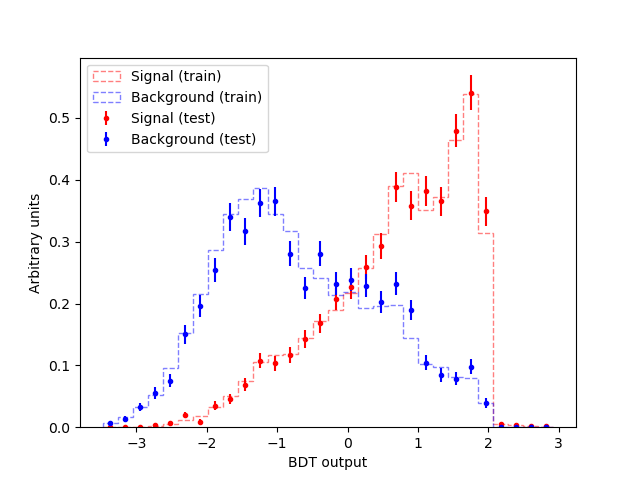
\includegraphics[scale=0.8]{overtrainingCheck.png}
	\centering
	\caption{Normalised histograms of the BDT discriminator output from the signal and background classes for the training and test sets.}
	\label{fig:bdt-overtrain-check}
\end{figure}

We can see that the shapes of the training and test sets for both signal and background are very similar. This is a good indicator that no overtraining occurred.




\section{Fake Lepton Estimation} 
Expected to be a small effect, why? Brief, general explanation/idea of methods used (full explanation/description of what we did and the results/plots/etc. later) 
\section{Analysis Pipeline/Workflow and TRExFitter}
What is TRExFitter? What can it do? At which stage(s) in the analysis did we use it? Which version did we use? Binning method. Explain calculation of error bars in TRF. \\\\ 
Include general flow chart of analysis (not sure where)

We make use of industry standard \texttt{ROOT}\footnote{CERN's HEP data analysis framework (written in C\texttt{++})} wrappers in this analysis, namely, \texttt{PyROOT} and \texttt{TRExFitter}.\\\\
\texttt{Python} is used extensively in many fields of science (not limited to physics and data science) due to its simplicity and ongoing support by the communities which utilize it. \texttt{PyROOT} allows users to access the full \texttt{ROOT} functionality within \texttt{Python}. More specifically, \texttt{PyROOT} provides \texttt{Python} bindings for \texttt{ROOT}.\\\\
\texttt{TRExFitter} is a framework for binned template profile likelihood fits\cite{TRexfitter}. In this analysis, we used TRExFitter (tag: \texttt{TRExFitter-00-04-11}) to produce all pre-fit and post-fit plots (including fit statistics, e.g. limit, significance, $\mu_{best-fit}$).\\\\
The analysis pipeline starts with sample derivations (derived dataset) being submitted to the grid for ntuple production. This applies cuts and selections to the already reduced derivations and produces ntuples with trees containing variables (e.g. scale factors, observables, MC truth flags) that will be used at future stages in the analysis. These ntuples are then read by \texttt{PyROOT} where the events are looped over, before being written to \texttt{ROOT} files as input to \texttt{TRExFitter}. The \texttt{Python} script's main purpose is to define the different regions and apply the final cuts and selections outlined in Table \ref{tab:4Lep-cutsummary}. As each event is looped over, these cut and selection criteria are checked for the given event and is either thrown away, or gets written to a \texttt{ROOT} file corresponding to the MC sample and Full Run 2 data-set (mc16a, mc16d, mc16e) which it belongs to. \texttt{TRExFitter} then takes these files as input, runs a maximum likelihood fit and produces relevant plots (e.g. pre-fit, post-fit, pull plots) and statistical parameters (e.g. limit, significance, $\mu_{best-fit}$).\\\\
Throughout this analysis, we ensured that the signal region was kept blinded. We did this by implementing \texttt{TRExFitter's} \textit{'mixed data and MC'}~\cite{MixedDataAndMC_TRF} fit, which aims to obtain the most accurate prediction for the expected results (while keeping the signal region blinded). It does this by performing a background only fit to the control regions (using real data). The set of fitted values for all the nuisance parameters from the background only fit are then used to construct a modified ASIMOV data-set. Finally, the fit is performed using real data in the control regions and the aforementioned modified ASIMOV data-set in the signal region.








